%\documentclass[reprint,amsmath,amssymb,superscriptaddress,prl,showpacs,onecolumn]{revtex4-1}
\documentclass[preprint,amsmath,amssymb,superscriptaddress,showpacs,pre]{revtex4-1}

\usepackage{graphicx}% Include figure files
\usepackage{dcolumn}% Align table columns on decimal point
\usepackage{bm}% bold math
\usepackage{color}
\usepackage{epstopdf} 
\usepackage{amsmath,amsfonts,amssymb,amsthm}
% \usepackage{hyperref}
\usepackage{algorithm}
\usepackage{algorithmic}
\usepackage{braket}
\usepackage[sans]{dsfont}
\usepackage{mathbbol}
\usepackage{bbm}

%% Added by Pierre
\usepackage{lineno}
\usepackage{nicefrac}       % compact symbols for 1/2, etc.
\usepackage{microtype}      % microtypography



\linenumbers

\DeclareMathOperator\atanh{arctanh}
\let\originalleft\left
\let\originalright\right
\renewcommand{\left}{\mathopen{}\mathclose\bgroup\originalleft}
\renewcommand{\right}{\aftergroup\egroup\originalright}
%\newcommand{\bra}[1]{\ensuremath{\left< #1\right|}}
%\newcommand{\ket}[1]{\ensuremath{\left|#1\right>}}
\newcommand{\ovl}[2]{\ensuremath{\left\langle #1\middle|#2\right\rangle}}
\newcommand{\ie}{\emph{i.e.}}
\newcommand{\eg}{\emph{e.g.}}
\newcommand{\cf}{cf.}
\newcommand{\cp}{\emph{cp.}}
%\newcommand{\braket}[2]{\left< #1,#2\right>}
%%\newcommand{\<}{\langle}
%%\renewcommand{\>}{\rangle}
\providecommand{\abs}[1]{\ensuremath{\left|#1\right|}}
\providecommand{\norm}[1]{||#1||}
\newcommand{\arctanh}[1]{\mathrm{arctanh}#1}
\newcommand{\Sign}[1]{\mathrm{Sign}#1}

\def\<{\langle}
\def\>{\rangle}
\def\vx{\vec x}
\def\vh{\vec h}

\newcommand{\ud}{\mathrm{d}}
\newcommand{\etal}{\textit{ et. al. }}
\newcommand{\Ham}{\mathcal{H}}
\newcommand{\B}{\beta}
\def\matF{{\mathbb F}}
\def\Jij{J_{ij}}

\def\Imat{\mathbb{I}}
\def\ext{\qopname\relax m{ext}}

\newcommand{\mi}{\mathrm{i}}
\DeclareMathOperator{\Tr}{Tr}

%%%% 

\newcommand{\ddroit}{\textrm{d}}
\newcommand{\Ptot}{P(A_1\ldots A_L)}
\newcommand{\xz}{\vec{x}_0}
\newcommand{\xo}{\vec{x}_1}
\newcommand{\xt}{\vec{x}_2}
\newcommand{\Lam}{\bm{\Lambda}}
\newcommand{\Sig}{\bm{\Sigma}}
\newcommand{\Sigmone}{\bm{\Sigma^{-1}}}
\def\fonetwo{\frac 1 2}
\def\Cmone{C^{-1}}
\def\Lambtwo{\Lambda^2} 
\def\tildex{\tilde{x}}
\newcommand{\HRule}{\rule{\linewidth}{0.5mm}}
\newcommand{\Xk}[1]{X^{\{#1\}}}
\newcommand{\xk}[1]{\vec{x}_{#1}}

% Pierre
\newcommand{\pierre}[1]{{\color{red}Pierre: #1}}
\newcommand{\curlynormalpar}[1]{\exp\left\{-\frac{1}{2}\left( #1 \right)\right\}}
\newcommand{\curlynormal}[1]{\exp\left\{-\frac{1}{2} #1 \right\}}
\newcommand{\iSig}{\bm{\Sigma^{-1}}}
\newcommand{\iC}{\bm{C}^{-1}}
\newcommand{\av}[1]{\left\langle #1 \right\rangle}
\newcommand{\vsa}{\vec{s}_a}
\newcommand{\vuka}{\vec{u}_{ka}}

\begin{document}

\title{Inference of global coevolutionary models from hierarchical correlated data.}
\date{}

\author{Edwin Rodriguez Horta} 
\affiliation{Group of Complex Systems and Statistical Physics, Department of Theoretical Physics, University of Havana, Cuba}
\affiliation{Laboratoire de Biologie Computationnelle et Quantitative (LCQB), Sorbonne Université, France}
%
\author{Pierre Barrat-Charlaix} 
\affiliation{Biozentrum, Universität Basel, Switzerland}
%
\author{Alejandro Lage} 
\affiliation{Group of Complex Systems and Statistical Physics, Department of Theoretical Physics, University of Havana, Cuba}
%
\author{Martin Weigt} 
\email{Correspondence to: Martin Weigt, \bf{martin.weigt@upmc.fr}}
\affiliation{Laboratoire de Biologie Computationnelle et Quantitative, Sorbonne Université, France}




\begin{abstract}
	The Inverse problem of Statistical Physics infers maximum-entropy  models  compatibles with a corresponding set of empirical averages extracted from a high-dimensional dataset of equilibrium configurations. Practical interest extended these methods to non-equilibrium data  like  time series, where detailed balance does not hold. However, in several applications, data samples  result from evolutionary processes and the relation between configurations is conditioned by a hierarchical structure of the population. This makes sample statistics a superposition of  signals coming from both: internal configuration correlations and relatedness correlations produced by common evolutionary  history, typically represented by a tree. How to disentangle both sources of correlation for a better parameter inference is an open question to explore. Here we propose an approach  where the  evolutive process through a phylogenetic tree is described by  a  multivariate Ornstein-Uhlenbeck dynamics characterized by  gaussian propagator and stationary distributions. Inference of these distributions from  phylogenetic non-independent samples is solved in a Bayesian framework. This procedure can be  extended to discrete variables by using a binary representation of data and approximating  binary sates by continuous variables. Our method proposes a possible way for  a better estimation of both, equilibrium and dynamic parameters, making  applications more accurate. 
\end{abstract}


\maketitle


\section{Introduction}
\label{sec:int}
Theory and applications of the inverse problem of statistical physics has had great development in recent years since the availability of large amounts of data on a microscopic scale produced by the continuous technological progress. In this context statistical physics paths: from model parameters to  observables, is reversed, toward find global models which describe the statistics of  a set of observed  configurations \cite{Inverse_problem_Berg}. 

Most of the work has been focus in equilibrium reconstruction , where the aim is to learn max Entropy models, Boltzman distribution, from independent and identically distributed equilibrium configurations. Another kind of methods deal with parameters learning from either time series data or from samples of the non-equilibrium steady state: non-equilibrium reconstruction.

Less effort has been done for data biased by population structured signal, where  samples  are not independent because of presence of relatedness between configurations. These structure could be for instance of  geographical or demogrhapic  nature in a population or  phylogenetic  nature  related to a evolutionary processes shaping trait variation among species.  Here we are going to deal with data given by sequences phylogenetically related  through a tree, which describes the hierarchical correlation between configurations. An important problem is the  distinction   of patterns induced by species traits or by phylogeny. 

Our source of inspiration came from the inverse problem in proteins \cite{Inverse_problem_proteins}, where  covariance signal present in an alignment of homologous proteins is described via Potts model. This covariance signal is assumed a consequence of phenotypics constraints like protein structure and function. However it is known that phylogeny relationships in homologous sequences  contaminate the statistics of  the alignment used to learn the equilibrium model. Therefore a direct inference on this alignments  leads to the existence of Potts parameters that attempt to model the full biased statistics limiting their capacity to predict phenotypic properties.

 To define and solve the inverse problem of statistical physics for data samples with hierarchical  relatedness structure is the aim of this work. 

Main difficulties to address  this kind of problem  come from the necessity to use  a proper global evolutionary model which describes the relation between sequences edge connected in a tree and the discrete  characters of data variables which makes certain calculations intractable \cite{entropy_paper}. 

Here we  adopt an approximation where we forget about the discrete nature of variables and model them by continuous variables instead. This transforms the Potts model into a Gaussian distribution \cite{Baldassi}, making the design of a global propagator tractable. We propose a model of evolution described by a multivariate Ornstein-Uhlenbeck process \cite{gardiner}, which is used  to generate evolutionary related data given an arbitrary phylogenetic tree. The corresponding inverse problem became in the inference of the Gaussian potential (Potts parameters) from the knowledge of tree leaves configurations and the dynamics of evolution. 

To this aim, we first review in section \ref{sec:ornstein_uhlenbeck_dynamics}, main characteristics of a multivariate Ornstein-Uhlenbeck process. In section \ref{evolutionary process} we describe the evolutionary process, describing the algorithm used to generate data phylogenetically biased. The statement of the problem in a Bayesian framework is shown in section \ref{statement of the problem}. Section \ref{methods} is dedicated to describe methodology used to solve the inverse problem. Results for evolution of continuos variable sequences and  the application for configuration of discrete variables is presented in section \ref{Results}. Finally the conclusion and outlook in \ref{conc}.



\section{The multivariate Ornstein-Uhlenbeck process}
\label{sec:ornstein_uhlenbeck_dynamics}

We consider a system characterized by $L$ continuous degrees of freedom and whose state is fully described by a vector $\vx$ of length $L$. 
These degrees of freedom can be continuous phenotypic traits of some living organism, or the sequence of a gene or a protein if a continuous approximation is made. 
At equilibrium, $\vx$ is normally distributed:
\begin{equation}
	P_{eq}(\vx) = \frac{1}{Z(\bm{J})}\curlynormal{\vx^T\bm{J}\vx},
	\label{eq:eq_distribution}
\end{equation}
where $\bm{J}$ is the symmetric positive definite \emph{coupling matrix} and $Z(\bm{J})$ is a normalization constant. 
We are interested in inferring this coupling matrix from a given amount of observed states $\vx$ of the system.
If these observations were independent from each other, $\bm{J}$ would simply be equal to the inverse of the \emph{covariance matrix} of the data, written $\bm{C}$. 

However, we are concerned here with the case where these observations are not independent. 
On the contrary, they are the result of a dynamical process which took place during a finite amount of time, and is thus not necessarily equilibrated. 
This dynamical process is described below.

We suppose that the considered system evolves according to the following Langevin equation 
\begin{equation}
	\gamma^{-1}\frac{\text{d}\vx}{\text{d}t} = - \bm{J}\vx + \vec{\xi}(t).
	\label{eq:langevin}
\end{equation}
Here, $\vec{\xi}(t)$ is a vector of uncorrelated white noises, and $\gamma^{-1}$ is the characteristic timescale governing the dynamics. 
In short, equation~\ref{eq:langevin} states that the system described by $\vx$ undergoes Brownian motion in an energy landscape characterized by the coupling matrix $\bm{J}$. 

We are not interested in $\vx$ directly, but rather by its probability distribution $P(\vx,t\vert\,\vx_0)$, that is the probability to find the system in state $\vx$ knowing it was in state $\vx_0$ and evolved for time $t$. 
The Fokker-Planck equation corresponding to equation~\ref{eq:langevin} is straightforward to write: 
\begin{equation}
	\gamma \partial_t P = \left(-\sum_{a,b=1}^L\frac{\partial}{\partial x_a} J_{ab}x_b + \sum_{a=1}^L\frac{\partial^2}{\partial x_a^2}\right) P, 
	\label{eq:FP}
\end{equation}
where the parenthesized expression on the right hand side is understood as an operator on $P$. 
The solution to~\ref{eq:FP} is a multivariate normal distribution~\cite{singh2017multiOU}:
\begin{equation}
	P(\vx, \Delta t|\, \vx_0) = \left((2\pi)^N\det\iSig\right)^{-1/2}
	\curlynormal{(\vx-\vec{\mu})^T\iSig(\vx- \vec{\mu})},
	\label{eq:OUpropagator}
\end{equation}
where we introduce matrices $\Sig$ and $\Lam$ as well as vector $\vec{\mu}$: 
\begin{equation}
	\Lam = e^{-\gamma\bm{J}}, \qquad \vec{\mu} = \Lam^{\Delta t} \vx_0, \qquad \Sig = \bm{J}^{-1}(\mathbb{1} - \Lam^{2\Delta t}).
	\label{eq:def_lambda}
\end{equation}
Equations~\ref{eq:OUpropagator} and~\ref{eq:def_lambda} define a multivariate \emph{Ornstein-Uhlenbeck} process (OU). 

It is important to note that since matrix $\Lam$  is the exponential of $-\bm{J}$, it is symmetric, has strictly negative eigenvalues and commutes with $\bm{J}$. 
We also underline the fact that $\Sig$ and $\vec{mu}$ depend on $\Delta t$, although this dependence is absent in our notation. 

By taking $\gamma\Delta t \gg 1$ and using the fact that $\bm{J}$ has strictly positive eigenvalues , one immediately recovers equation~\ref{eq:eq_distribution}. 
This allows us to compute the joint distribution of two configurations $\vx_1$ and $\vx_2$ separated by a time $\Delta t$ by multiplying equations~\ref{eq:eq_distribution} and~\ref{eq:OUpropagator}: 
\begin{equation}
	P(\vx_1, \vx_2\vert\,\Delta t) \propto \curlynormalpar{\vx_1^T\iSig\vx_1 + \vx_2^T\iSig\vx_2 - 2\vx_1^T\Lam^{\Delta t}\iSig\vx_2}. 
	\label{eq:OUjoint}	
\end{equation}
This last equation is important as it allows one to compute the joint covariance of configurations $\vx_1$ and $\vx_2$. 
The probability distribution in~\ref{eq:OUjoint} is a normal distribution whose inverse covariance matrix is defined by blocks: $\Sig$ on the diagonal and $-\Lam^{\Delta t}\Sig$ off-diagonal. 
By inverting this block matrix, given that $\Lam$ and $\Sig$ commute and are invertible, one obtains the following covariance: 
\begin{equation}
	\langle \vx_1\vx_2^T \rangle_{\Delta t} = \Lam^{\Delta t}\bm{J}^{-1} = \Lam^{\Delta t}\bm{C}. 
	\label{eq:pairwisecov}
\end{equation}
As said above, the aim of this work is to infer matrix $\bm{J}$ from a set of observations $\vx$ that are generated this OU process. 
More precisely, any two observations $\vx_1$ and $\vx_2$ will be separated by a time $\Delta t$ during which the OU process took place. 
Equation~\ref{eq:pairwisecov} then allows us to distinguish two regimes. 
Let us call $\{\rho_a\}$ the eigenvalues of $\bm{J}$. 
Using the definition of $\Lam$, we immediatly have that the eigenvalues of matrix $\Lam^{\Delta t}\bm{C}$, \ie  the left hand side of equation~\ref{eq:pairwisecov}, are of the form $\rho_a^{-1}e^{-\gamma\rho_a\Delta t}$.

Since the $\rho_a$ are positive, the eigenvalues of $\Lam^{\Delta t}\bm{C}$ vanish exponentially for large enough times. 
The timescale of this exponential decrease is set by the characteristic time $\tau_c^{-1} = \gamma\rho_{min}$, where $\rho_{min}$ is the smallest eigenvalue of $\bm{J}$. 
Thus, for $\Delta t / \tau_c \gg 1$, $\vx_1$ and $\vx_2$ are uncorrelated. 
If this is verified for all pairs of observations, the regime is that of \emph{weakly correlated} data, and the inference of $\bm{J}$ can simply be performed by inverting the empirical correlation matrix. 
Inversely, for $\Delta t / \tau_c \ll 1$, $\vx_1$ and $\vx_2$ are highly correlated, defining a \emph{strongly correlated} regime. 
It should be noted that when $\Delta t = 0$, the joint correlation matrix of $\vx_1$ and $\vx_2$ becomes non invertible, and equation~\ref{eq:pairwisecov} becomes irrelevant. 






\section{Statement of the problem}
\label{statement of the problem}

\begin{figure}[!htb]
	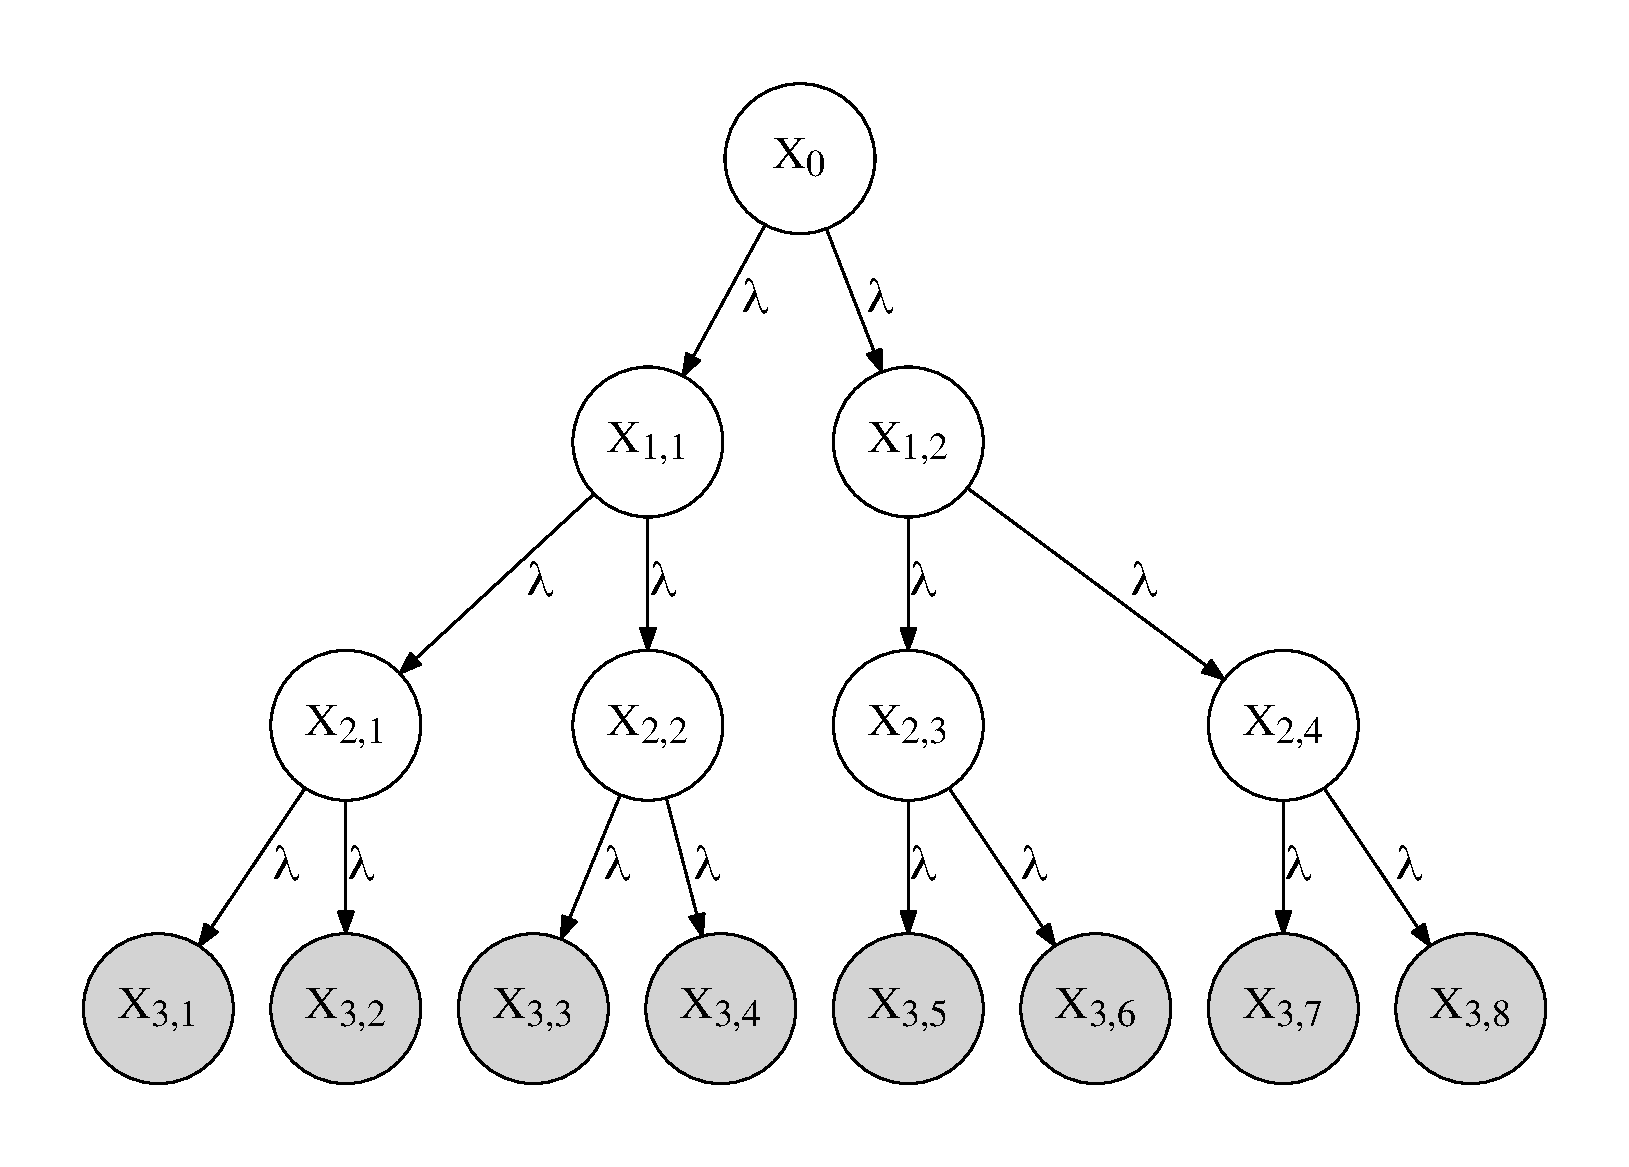
\includegraphics[width=0.6\textwidth]{Figures/tree.pdf}
	\caption{ \pierre{We should get a better figure here.}}
	\label{fig:sample_tree}
\end{figure}


The central problem discussed here is the inference of the probability distribution describing samples that are hierarchically correlated by a tree. 
Formally, we assume that the data consists of $N$ real valued vectors of length $L$, noted $\{\vx_i\}$ with $i\in\{1\ldots N\}$. 
Taken individually, the $\vx_i$s are normally distributed according to equation~\ref{eq:eq_distribution}. with mean $0$.
By construction, the equilibrium correlation between components of vectors $\vx$ is given by the inverse of the couplings, that is $\langle x^a x^b\rangle-\langle x^a\rangle\langle x^b\rangle = \bm C_{ab} = (\bm J^{-1})_{ab}$. 
This implies that inferring the coupling matrix defining the probability distribution amounts to finding the \emph{equilibrium} covariance matrix $\mathbf{C}$.  

However, this covariance cannot be directly measured as we consider observations that are not independently distributed.
Instead, the set of measured configurations $\{\vx_i\}$ is the result of an Ornstein-Uhlenbeck (OU) process taking place on a tree $\mathcal{T}$, such as the one shown in figure~\ref{fig:sample_tree}. 
The configuration $\vx_i$ of each node $c$ in the tree is the result of the evolution given by the equation~\ref{eq:langevin}, with initial condition $\vx_{a(i)}$, $a(i)$ being the ancestral node of $i$, and running time $\Delta t_{ia(i)}$, that is the \emph{branch length} between $a(i)$ and $i$. 
This process is initialized with a root note $\vx_r$ that is distributed according to equation~\ref{eq:eq_distribution}.
Observed data points are leaves of this tree, which is assumed to be perfectly known.
The nature of the chosen evolution process implies that the distribution of a leaf configuration $\vx_i$ conditioned on the knowledge of another leaf configuration $\vx_j$ is given by equation~\ref{eq:OUpropagator}, where $\Delta t=\Delta t_{ij}$ represents the total branch length separating leaf $i$ and leaf $j$.

The OU process is fully characterized by the quadratic potential $\bm J = \bm C^{-1}$ and a rate $\gamma$. 
Hence, the configurations of the leaves, that is the data, are determined only by $\bm C$, $\gamma$, and the tree $\mathcal{T}$. 
The aim of this work is to design a method to infer the most likely values of $\bm C$ and $\gamma$ from the knowledge of the data $\mathcal{D}=\{\vx_i\}$ and the shape of $\mathcal{T}$. 
There are two notable extreme cases to this problem. 
The first one is the $\Delta t_r/\tau_c\longrightarrow 0$ case, where $\Delta t_r$ is the typical branch length distance from leaves to root. 
Leaf configurations are then almost identical to the root, \emph{i.e.} $\vx_i\simeq\vx_r$, and inference of $\bm C$ becomes impossible. 
The second one is the $\Delta t_r/\tau_c\longrightarrow\infty$ case, where equilibration of the OU process takes place almost instantly when compared to branch lengths of $\mathcal{T}$.
Leaf configurations are then independently drawn from the equilibrium distribution $P_{eq}$, and $\bm C$ can be readily estimated from the empirical covariances. 
Here, we deal with the intermediary cases where the tree makes it impossible to simply estimate $\bm C$ from empirical covariances, but where $\tau_c$ is not large enough to remove all signatures of the energy potential. 

We adopt a Bayesian approach to this inference problem by writing the probability of a given set of parameters as a function of the data using the following relation
\begin{equation}
	P(\bm C, \gamma\vert\mathcal{D},\mathcal{T}) \propto P(\mathcal{D}\vert\bm C, \gamma,\mathcal{T})\cdot P(\bm C, \gamma),
	\label{eq:bayesian_likelihood}
\end{equation}
where the proportionality constant does not depend on the parameters $\bm C$ or $\gamma$, and where $P(\bm C, \gamma)$ can be any arbitrarily chosen prior distribution. The difficulty in equation~\ref{eq:bayesian_likelihood} lies in the estimation of the term $P(\mathcal{D}\vert\bm C, \gamma, \mathcal{T})$, that is the likelihood of the data given a set of parameters $\bm C$ and $\gamma$ and the tree $\mathcal{T}$.  We detail the computation of this likelihood in the following section. 

\subsection{Calculation of the likelihood} % (fold)
\label{sub:Calculation_of_the_likelihood}
 
The joint distribution of two configurations $\vx_1$ and $\vx_2$ separated by time $\Delta t$ is given by equation~\ref{eq:OUjoint} and corresponds to a joint normal distribution. 
This means that the vector $\vec{X}=[\vx_1, \vx_2]$, \emph{i.e.} the concatenation of vectors $\vx_1$ and $\vx_2$, follows a normal distribution with null means.
Of importance here is that this property of the OU process can be extended to the joint distribution of any subset nodes in a tree. 
In other words, if we now define $\vec{X}=[\vx_1,\ldots,\vx_N]$ to be the concatenation of the configurations of all leaves of $\mathcal{T}$, we can write the distribution of $\vec{X}$ as
\begin{equation}
	P(\vec{X}\vert\,\bm{C},\gamma,\mathcal{T}) = \left((2\pi)^{LN}\det\mathbb{G}\right)^{-\frac{1}{2}}\curlynormal{\vec{X}^T\mathbb{G}^{-1}\vec{X}},
	\label{eq:multiOU_jointall}
\end{equation}
where $\mathbb{G}$ is the \emph{joint correlation matrix} and depends on the tree as well as on $\bm{C}$ and $\gamma$.
This property is shown in more detail in section \ref{sec:joint_probability_of_leaves_is_a_gaussian} of the Supplementary Material.\\
Equation~\ref{eq:multiOU_jointall} allows us to compute the log-likelihood of the data $\vec{X}$ as a function of $\vec{X}$ itself and of the joint correlation matrix. 
Indeed, taking its logarithm immediatly gives
\begin{equation}
	\mathcal{L}_{\mathcal{D}}(\mathbb{G}) = -\frac 1 2 \log \det  \mathbb{G}  -\frac 1 2 \vec{X}^T\mathbb{G}^{-1} \vec{X} + \text{cte}. 
	\label{eq:likelihood_2}
\end{equation}

We will now use the fact that the joint distribution of the leaves is a Gaussian to compute $\mathbb{G}$ as a function of the tree and the parameters of the OU process.
The joint correlation matrix is of dimensions $(L\cdot N)\times(L\cdot N)$ where $L$ is the length of individual Gaussian vectors $\vx_i$. 
It describes the correlation of each leaf of the tree to every other leaf, in the sense that the $L\times L$ block $\mathbb{G}_{ij}$ with $1\leq i,j\leq N$ corresponds to the covariance of configurations $\vx_i$ and $\vx_j$. 
In other words, for indices $a$ and $b$ such that $1\leq a,b\leq L$, we have
\begin{equation}
	\mathbb{G}_{ij}(a,b) = \av{x_i^a x_j^b}. 
	\label{eq:jointcov_1}
\end{equation}
Since $\vx_i$ and $\vx_j$ are leaves of the tree, they are separated by an evolution of the OU proces for a time $\Delta t_{ij}$.
This means that without knowledge of the internal nodes, $\vx_i$ and $\vx_j$ are distributed according to equation~\ref{eq:OUjoint}. 
In particular, this implies that their covariance matrix is given by equation \ref{eq:pairwisecov}.
From this we can derive the value of the block $(i,j)$ of the joint correlation matrix, obtaining the following equation for $\mathbb{G}$: 
\begin{equation}
	\mathbb{G}_{ij} =
	\begin{cases}
		\bm C & \text{if $i=j$}.\\
		\Lam^{\Delta t_{ij}}{\mathbf{C}} & \text{otherwise}  
	\end{cases}.
	\label{eq:jointcov_2}
\end{equation}
We remind here that $\Lam = e^{-\gamma\iC}$ depends only on $\gamma$ and $\mathbf{C}$, and commutes with $\mathbf{C}$.  \\


We can now use the structure of $\mathbb{G}$ described in equation~\ref{eq:jointcov_2} to re-write equation~\ref{eq:likelihood_2} in a way that we can compute. 
More precisely, we will attempt to write the likelihood as a function of eigenmodes of $\iC$. \\
Let us first note $\left\{\rho_a, \vsa\right\}$ the eigenvalues and eigenvectors of $\iC$, where the index $a$ runs from $1$ to $L$ and vectors $\vsa$ are of dimention $L$. 
By definition, we have $\rho_a>0$ for all $a$.  
The properties of the exponential of matrices imply that vectors $\vsa$ are also eigenvectors of the matrix $\Lam$. 
Thus, we can easily write the eigenmodes of the block $\mathbb{G}_{ij}$ as $\left\{z(\rho_a, \Delta t_{ij}), \vsa\right\}$ where we introduced
\begin{equation}
	z(\rho_a, \Delta t_{ij}) = \rho_a^{-1}e^{-\gamma\rho_a\Delta t_{ij}}.
	\label{eq:z}
\end{equation}
By convention, $\Delta t_{ii} = 0$ and $z(\rho_a, \Delta t_{ii}) = \rho_a^{-1}$. \\
We also introduce matrix $\mathbf{G}^a$ of dimensions $N\times N$ and defined for indices $1\leq i,j\leq N$ as 
\begin{equation}
	\mathbf{G}^a_{ij} = z(\rho_a, \Delta t_{ij}). 
	\label{eq:subG_def}
\end{equation}
In other words, for a given index $1\leq a\leq L$, $\mathbf{G}^a$ is the matrix built by replacing blocks of $\mathbb{G}$ by their $a$th eigenvalue.
Matrices $\mathbf{G}^a$ are symmetric have their own eigenmodes, that we note $\left\{\lambda_{ka}, \vuka\right\}$ with $k$ running from $1$ to $N$.

To obtain the eigenmodes of $\mathbb{G}$ as a function of the $\vsa$ and $\vuka$, we construct the \emph{Kronecker} product of vectors $\vsa$ and $\vuka$, defining vectors $\vec{S}_{ka}$ of dimension $L\times N$: (\pierre{should we say tensor product? I had never heard of Kronecker product before... I'm fine with it, but people might be more familiar with tensor?})
\begin{equation}
	\begin{split}
		\vec{S}_{ka} &= \vuka \otimes \vsa \\
		&= [u_{ka}^1\cdot\vsa, \ldots, u_{ka}^N\cdot\vsa].
		% &= [u_{ka}(1)s_a(1), \ldots, u_{ka}(1)s_a(L); \ldots; u_{ka}(N)s_a(1), \ldots, u_{ka}(N)s_a(L)]
	\end{split}
	\label{eq:Sdef}
\end{equation}
The $i$th block vector of $\vec{S}_{ka}$ will be written as $\vec{S}_{ka}^i = u_{ka}^i\cdot\vsa$. 
We can now show that $\vec{S}_{ka}$ are eigenvectors of matrix $\mathbb{G}$ by considering the $i$th block vector of the product $\mathbb{G}\cdot\vec{S}_{ka}$:
\begin{equation}
	\begin{split}
		\left(\mathbb{G}\cdot\vec{S}_{ka}\right)^i &= \sum_{j=1}^N \mathbb{G}_{ij} u_{ka}^j\cdot\vsa \\
		&= \sum_{j=1}^N z(\rho_a, \Delta t_{ij}) u_{ka}^j\cdot \vsa \\
		&= (\mathbf{G}^a\cdot\vuka)^i \cdot \vsa\\
		&= \lambda_{ka}(u_{ka}^i\cdot\vsa) \\
		&= \lambda_{ka}\vec{S}_{ka}^i,
	\end{split}
\end{equation}
where we have first used the fact that $\vsa$ is an eigenvector of $\mathbb{G}_{ij}$, then the definition of $\mathbf{G}^a$, and finally the fact that $\vuka$ is an eigenvector of $\mathbf{G}^a$.
This shows that the eigenmodes of $\mathbb{G}$ are $\left\{ \lambda_{ka}, \vec{S}_{ka} \right\}$ with $1\leq k\leq N$ and $1\leq a \leq L$. 
Since $\mathbb{G}$ is the covariance matrix of a Gaussian distribution, we also obtain that the $\lambda_{ka}$ are strictly positive.

Equation~\ref{eq:likelihood_2} can now be rewritten using the eigen-decomposition of $\mathbb{G}$: 
\begin{equation}
	\begin{split}
		\mathcal{L}_{\mathcal{D}}(\mathbb{G}) &= -\frac 1 2 \sum_{k=1}^N\sum_{a=1}^L \log\lambda_{ka} - \frac 1 2 \sum_{k=1}^N\sum_{a=1}^L \lambda_{ka}^{-1}(\vec{X}\cdot \vec{S}_{ka})^2\\
		&= -\frac 1 2 \sum_{k,a} \left(\log\lambda_{ka} + \lambda_{ka}^{-1}	\left(\sum_{i=1}^N u_{ka}^i\vx_i\cdot\vsa\right)^2 \right).
	\end{split}
	\label{eq:likelihood_3}
\end{equation}
Equation~\ref{eq:likelihood_3} expresses the likelihood as a function of $\vuka$, $\lambda_{ka}$ and $\vsa$. 
However, the definition of matrix $\mathbf{G}^a$ given by equation~\ref{eq:subG_def} makes clear that its eigenmodes $\{\lambda_{ka}, \vuka \}$ depend only of the eigenvalues $\rho_a$ of $\iC$, on $\gamma$, as well as of the structure of the tree through the quantities $\Delta t_{ij}$, although this dependence cannot be analytically expressed in a simple manner. 
This means that the likelihood in equation~\ref{eq:likelihood_3} is in fact a function of $\{\rho_a, \vsa\}$, \emph{i.e.} the eigenmodes of $\iC$ and of the time scale parameter $\gamma$.



% subsection derivation_of_the_likelihood (end) 

\subsection{Maximization of the likelihood} % (fold)
\label{sub:maximization_of_the_likelihood}

As stated at the beginning of this section, our main task is to find the equilibrium covariance matrix $\mathbf{C}$ that maximizes the likelihood of the data. 
We also need to find the optimal time scale $\gamma$. 
In equation~\ref{eq:likelihood_3}, the likelihood is expressed as a function of $\gamma$ and $\{\rho_a, \vsa\}$, \emph{i.e.} the eigenvalues and eigenvectors of $\iC$, either directly or through the quantities $\{\lambda_{ka}, \vuka \}$. 
We know attempt to maximize the likelihood with respect to the eigenmodes $\{\rho_a, \vsa\}$ and $\gamma$. \\
In order to perform this optimization, we will need to conduct optimization with the eigenvectors $\{\vsa\}$ as a variable. 
Since $\iC$ is a symmetric matrix, its eigenvectors form an orthogonal basis of the vector-space of dimension $L$. 
Thus, they are fully characterized by $L(L-1)/2$ scalar \emph{Eulerian angles} $\{\theta_{\alpha\beta}\}$ with $1\leq \alpha < \beta \leq L$~\cite{Raffenetti1970GEA}(\pierre{\cite{Shepard_param_OM} was cited as well, do we keep it?}). 
We will use these Eulerian angles to parametrize the $\{\vsa\}$. The $\{\theta_{\alpha\beta}\}$ along with the $L$ eigenvalues $\rho_a$ allow to fully parametrize the $L(L+1)/2$ distinct values of $\iC$. \\

We now set to computing the gradient of the likelihood $\mathcal{L}_{\mathcal{D}}(\mathbb{G})$ with respect to parameters $\{\rho_a, \theta_{\alpha\beta}\}$ and $\gamma$. 
To make explicit the dependence of eigenvalues and eigenvectors of matrices $\mathbf{G}^a$ with respect to these parameters, we introduce the notation $\vec{u}_k(\rho_a,\gamma) = \vuka$ and $\lambda_k(\rho_a,\gamma) = \lambda_{ka}$. 
Note that from the definition of $\mathbf{G}^a$ in equation~\ref{eq:subG_def}, its eigenvalues and vectors depend only on the eigenvalues of $\iC$ and not on its eigenvectors. 
In the same way, we will now write $\mathbf{G}(\rho_a,\gamma)$ instead of $\mathbf{G}^a$. \\
The gradient of the likelihood is obtained by differentiating equation~\ref{eq:likelihood_3} with respect to parameters of interest. 
This gives us  three equations for the gradient: 
% dL / d rho
\begin{equation}
	\begin{split}
		\frac{\partial \mathcal{L}}{\partial\rho_a} &= -\frac 1 2 \sum_{k=1}^N \left\{ \frac{\partial\lambda_k}{\partial\rho_a}\lambda_k^{-1} - \frac{\partial\lambda_k}{\partial\rho_a} \lambda_k^{-2}\left(\sum_{i=1}^N u_{k}^i\vx_i\cdot\vsa\right)^2 \right. \\
		&+ \left. 2\lambda_k^{-1} \left(\sum_{i=1}^N u_k^i\vx_i\cdot\vsa\right) \left(\sum_{i=1}^N \frac{\partial u_k^i}{\partial\rho_a} \vx_i\cdot\vsa\right) \right\}, 
	\end{split}
	\label{eq:gradlikelihood_1}
\end{equation}
% dL / d theta
\begin{equation}
	\frac{\partial \mathcal{L}}{\partial\theta_{\alpha\beta}} = \sum_{k=1}^N \lambda_k^{-1} \left(\sum_{i=1}^N u_k^i\vx_i\cdot\vsa\right) \left(\sum_{i=1}^N u_k^i \vx_i\cdot\frac{\partial \vsa}{\partial\theta_{\alpha\beta}}\right),
	\label{eq:gradlikelihood_2}
\end{equation}
and
% dL / d gamma
\begin{equation}
	\begin{split}
		\frac{\partial \mathcal{L}}{\partial\gamma} &= -\frac 1 2 \sum_{k=1}^N \left\{ \frac{\partial\lambda_k}{\partial\gamma}\lambda_k^{-1} - \frac{\partial\lambda_k}{\partial\gamma} \lambda_k^{-2}\left(\sum_{i=1}^N u_{k}^i\vx_i\cdot\vsa\right)^2 \right. \\
		&+ \left. 2\lambda_k^{-1} \left(\sum_{i=1}^N u_k^i\vx_i\cdot\vsa\right) \left(\sum_{i=1}^N \frac{\partial u_k^i}{\partial\gamma} \vx_i\cdot\vsa\right) \right\}, 
	\end{split}
	\label{eq:gradlikelihood_3}
\end{equation}
The derivatives of $\vec{u}_k(\rho,\gamma)$ and $\lambda_k(\rho,\gamma)$ with respect to $\rho$ can then be computed using the following equations~\cite{matrix_cook_book}: 
\begin{equation}
	\frac{\partial\lambda_i(\rho,\gamma)}{\partial\rho} = \vec{u}_k(\rho,\gamma)^T\frac{\partial\mathbf{G}(\rho,\gamma)}{\partial\rho}\vec{u}_k(\rho,\gamma)
	\label{eq:grad_eigval}
\end{equation}
and
\begin{equation}
	\frac{\partial \vec{u}_k(\rho,\gamma)}{\partial\rho} = \sum_{l\neq k} \left( \vec{u}_k(\rho,\gamma)^T\frac{\partial\mathbf{G}(\rho,\gamma)}{\partial\rho}\vec{u}_l(\rho,\gamma) \right) \left(\lambda_k(\rho,\gamma) - \lambda_l(\rho,\gamma)\right)^{-1} \vec{u}_l(\rho,\gamma).
	\label{eq:grad_eigvec}
\end{equation}
Equivalent equations can be written for their derivatives with respect to $\gamma$. 
\pierre{So what if we some eigenvalues cross?}.\\
The computation of the gradient of $\mathcal{L}$ for a given set of parameters $\{\rho_a, \theta_{\alpha\beta}\}$ then goes as follows. 
For each eigenvalue $\rho_a$, we compute and diagonalize matrix $\mathbf{G}(\rho_a)$ to obtain its eigenmodes $\vec{u}_k(\rho_a)$ and $\lambda_k(\rho_a)$. 
Using equations~\ref{eq:grad_eigval} and ~\ref{eq:grad_eigvec} and their equivalent form for $\gamma$, we also numerically compute their derivatives with respect to $\rho_a$ and $\gamma$. 
This gives us all the quantities to estimate the gradient of $\mathcal{L}$ with respect to $\rho_a$ using equation~\ref{eq:gradlikelihood_1}. \\

 This nonlinear optimization problem was addressed by implementing a quasi-Newton Method algorithms \cite{NLopt}. \pierre{More details about this would be great. }


% subsection maximization_of_the_likelihood (end)


\section{ Results}
\label{Results}
We base the test of methodology developed on a sampling-inference procedure defined by two steps: 
\begin{enumerate}
\item  Generation of simulated  data using   a non-homogeneous  tree in algorithm \ref{alg_1}  with initial parameters $\gamma_{init}$ and $\bm J_{init}$. The tree structure  used is  binary with $K=10$ levels and   branch length randomly selected in $(0,1)$ interval.
\item Inference procedure by maximizing Equation~\ref{eq:likelihood_3} finding the maximum likelihood estimators $\gamma_{max}$ and $\bm J_{max}$  . 
\end{enumerate}  

As was explained in section \ref{evolutionary process} , phylogenetic bias present at leaves of the tree depend of the set of time branch lengths  $\Delta t_{ij}$, the mutation rate $1/\gamma$ and the potential $\bm J$. This mean that in our simulations given the tree structure and $\bm J=\bm J_{init}$  we could define a threshold value for $\gamma$ above which  sequences in the  alignment are considered  non-independent: $\gamma_c=\lambda_{max}  \Delta t_{max}$, where  $\lambda_{max}$ is the maximum eigenvalue of $\bm J_{init}$ and $\Delta t_{max}$ is the  higher path time between two leaves in the tree.   Tunning the mutation rate respect $1/\gamma_c$ allow to generate sequences with distinct levels of phylogenetic bias. We choose three different values of parameter $\gamma$ in order to simulate  different regimes: with weak  $\gamma_{init}=0.1\gamma_c$ ,intermediate $\gamma_{init}=0.3\gamma_c$ and  strong  $\gamma_{init}=0.5\gamma_c$  phylogenetic signal. 

In order to limit the influence of a particular selection of the initial conditions in our simulations,  30 repetitions with different set of initial parameters were made.  Sequences with length $L=10$  was drawn in the root from a Gaussian distribution $P^0(\mathbf{ x})\sim N(0,\bm J_{init}^{-1})$. The different couplings matrices for each data generation was selected as a positive semidefinite matrix drawn from a normal distribution with mean $\mu_{J_{init}}=0.8$ and standard deviation $\sigma_{J_{init}}=0.2$. To make the matrix sparse we dilute the couplings with density $0.3$. 

In figures \ref{results_gamma10_n10},  \ref{results_corr_map_J_10_n10}, \ref{results_corr_map_C_10_n10} we compare the maximum likelihood estimators with the empirical ones which were obtained  from the inversion of the empirical covariance matrix ($\bm J_0=\bm C^{-1}_0$) and from minimization of the expression \ref{gamma_inverse_eq} on the parameter $\gamma_0$.  As can be seen    our method is able of inferring covariance and  coupling matrices closer to the initial  ones for all regimes, and  differences are more clear if there is more phylogenetic contamination in  alignments. 


On the other hand we wonder if our inference algorithm make a difference in the task of  reproduce the topology of the co-evolutionary network defined by Hamiltonian \ref{eq:equil}, identifying the strong pairs. As our original coupling matrix is sparse  we could explore the ability of maximum likelihood estimators to identify the strongest non-zero entries of the original coupling matrix $\bm J_{init}$.  Figure \ref{PPV_n10} show , for different levels of phylogeny contamination,  positive predictive values averaged over 30 samples. Comparison with the corresponding result from empirical estimators  shows that taking phylogeny into account, as is the case of our inference algorithm, also helps in this direction.


\begin{figure*}[!htb]
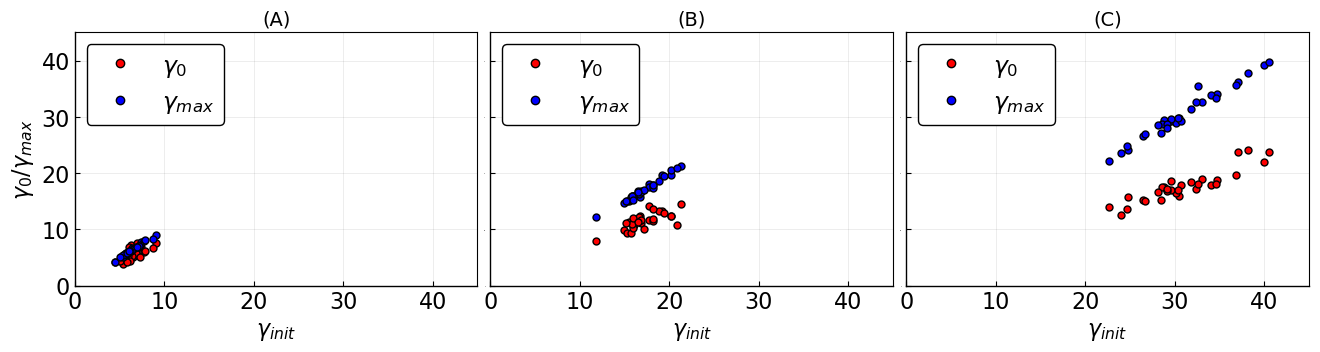
\includegraphics[keepaspectratio=true,width=1.0\textwidth]{Figures/gamma_panel_L10_M1024.png}
	\vspace{-1mm}
\caption{{ Results of inference of the  maximum likelihood ($\gamma_{max}$) and empirical ($\gamma_{0}$)  estimators of parameter $\gamma$. Each point correspond to a different sampling-inference process as result of simulations with different initial parameters: $\gamma_{init},\bm J_{init}$. The length of the sequence vectors was $L=10$ and the number of sequences  $M=1024$ as consequence of a binary non-homogeneous tree with $K=10$ levels. Three different regimes were explored incrementing from left to right the  phylogenetic bias present at leaves sequences where \textbf{A}: weak phylogenetic signal and   $\gamma_{init}=0.1*\gamma_c$, \textbf{B}: intermediate phylogenetic signal  and $\gamma_{init}=0.3*\gamma_c$, \textbf{C}: strong phylogenetic signal and $\gamma_{init}=0.5*\gamma_c$. }} \label{results_gamma10_n10}
\end{figure*}
	
\begin{figure*}[!htb]
	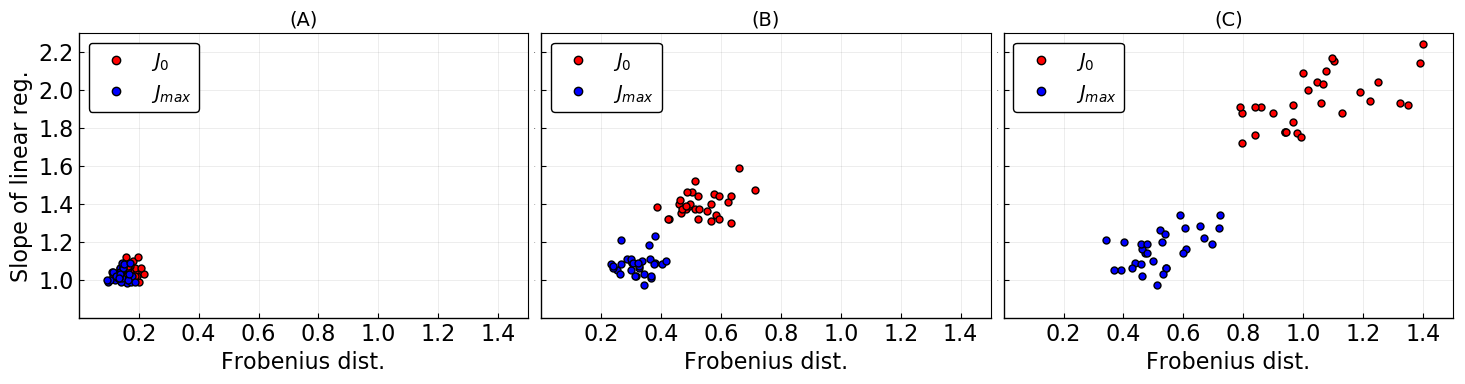
\includegraphics[keepaspectratio=true,width=1.0\textwidth]{Figures/couplings_panel_frob_dist_vs_lin_reg_slope_L10_M1024_same_range.png}
\vspace{-1mm}
\caption{{ Fobenious distance and  slope of linear regression between empirical ($\bm J_{0}$) / inferred couplings matrix ($\bm J_{max}$) and initial couplings matrix $\bm J_{init}$.  Each point correspond to a different sampling-inference process as result of simulations with different initial parameters: $\gamma_{init},\bm J_{init}$. The length of the sequence vectors was $L=10$ and the number of sequences  $M=1024$ as consequence of a binary non-homogeneous tree with $K=10$ levels. Three different regimes were explored incrementing from left to right the  phylogenetic bias present at leaves sequences where \textbf{A}: weak phylogenetic signal and   $\gamma_{init}=0.1*\gamma_c$, \textbf{B}: intermediate phylogenetic signal  and $\gamma_{init}=0.3*\gamma_c$, \textbf{C}: strong phylogenetic signal and $\gamma_{init}=0.5*\gamma_c$.}} 
\label{results_corr_map_J_10_n10}
\end{figure*}	
	
\begin{figure*}[!htb]
	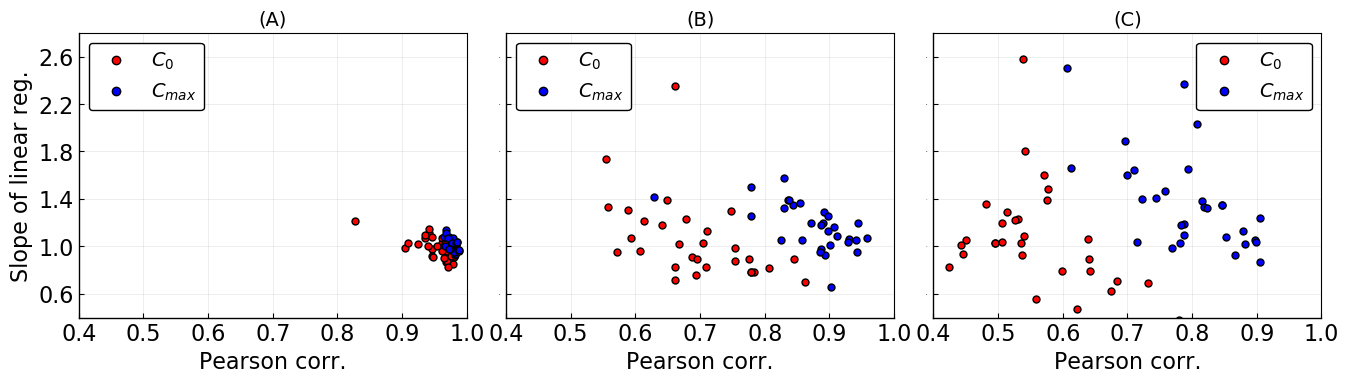
\includegraphics[keepaspectratio=true,width=1.0\textwidth]{Figures/covariance_panel_pearson_corr_vs_lin_reg_slope_L10_M1024_same_range.png}
	\vspace{-1mm}
\caption{{  Pearson correlation and  slope of linear regression between empirical ($\bm C_{0}$) /inferred ($\bm C_{max}$) covariance  matrix and to  initial covariance matrix $\bm C_{init}=\bm J^{-1}_{init}$.  Each point correspond to a different sampling-inference process as result of simulations with different initial parameters: $\gamma_{init},\bm J_{init}$. The length of the sequence vectors was $L=10$ and the number of sequences  $M=1024$ as consequence of a binary non-homogeneous tree with $K=10$ levels. Three different regimes were explored incrementing from left to right the  phylogenetic bias present at leaves sequences where \textbf{A}: weak phylogenetic signal and   $\gamma_{init}=0.1*\gamma_c$, \textbf{B}: intermediate phylogenetic signal  and $\gamma_{init}=0.3*\gamma_c$, \textbf{C}: strong phylogenetic signal and $\gamma_{init}=0.5*\gamma_c$.    \textbf{center}: $\gamma=\gamma_i$, \textbf{right} $\gamma=\gamma_s$.  }} 
\label{results_corr_map_C_10_n10}
\end{figure*}		


\begin{figure*}[!htb]
	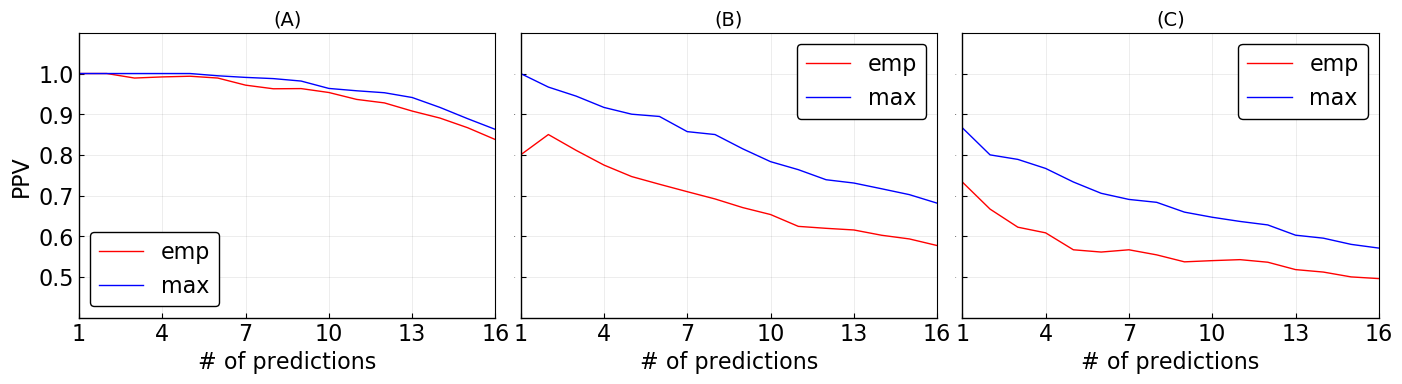
\includegraphics[keepaspectratio=true,width=1.0\textwidth]{Figures/PPV_panel_L10_M1024.png}
	\vspace{-1mm}
\caption{{  Positive predictive values (PPV) averaged over 30 samples,  for each of the three different regimes: \textbf{A}: weak phylogenetic signal and   $\gamma_{init}=0.1*\gamma_c$, \textbf{B}: intermediate phylogenetic signal  and $\gamma_{init}=0.3*\gamma_c$, \textbf{C}: strong phylogenetic signal and $\gamma_{init}=0.5*\gamma_c$.  Positive predictive values are found as a proportion of agreement in the strongest couplings of the matrix $\bm J_{init}$ . The length of the sequences was $L=10$ so that couplings matrix has $10^2$ entries of which on average only 16 off diagonals elements  are nonzero  given the sparse character of the initial matrices. }} .
\label{PPV_n10}
\end{figure*}		



\section{Discussion}
\label{sec:discussion}

\textbf{Acknowledgments:} 





\clearpage
\bibliography{bib_phylo}

\bibliographystyle{unsrt}

\newpage
\appendix
\setcounter{figure}{0}
\renewcommand{\figurename}{Figure S}
\setcounter{table}{0}
\renewcommand{\tablename}{Table S}

\section{Supplementary material} % (fold)
\label{sec:supplementary_material}


\subsection{Generating artificial data} % (fold)
\label{sub:generating_artificial_data}

	We are interested in the case where the described Ornstein-Uhlenbeck process takes place on a tree. 
	For example, if configurations $\vec{x}$ represent quantitative traits of some organisms, the tree can represent the genealogy or phylogeny of these organisms. 
	Therefore, we have to be able to simulate the OU process on a tree. 
	In practice, given a rooted tree such as the one shown in figure~\ref{fig:sample_tree} of the main text, we want to sample a configuration $\vec{x}$ for every node in such a way that equation~\ref{eq:OUjoint} holds for every pair of nodes, the time $\Delta t$ then being the branch length connecting them. \\
	We use a simple methodology to achieve this. 
	First, note that given an arbitrary configuration $\vec{x}_0$ and a time $\Delta t$, we can generate a new configuration $\vec{x}$ distributed according to the propagator in equation~\ref{eq:OUpropagator} by the transformation
	\begin{equation}
		\vx = \Lam^{\Delta t}\vx_0 + \Sig^{1/2}\vec{\eta}
		\label{eq:OUsample}
	\end{equation}
	where $\Lam$ and $\Sig$ are defined in equation~\ref{eq:def_lambda}, and $\vec{\eta}$ is a vector of uncorrelated variables with distributions $\mathcal{N}(0,1)$. 
	Moreover, if $\vec{x_0}$ is distributed according to equation~\ref{eq:eq_distribution}, then $\vx$ and $\vx_0$ are distributed according to equation~\ref{eq:OUjoint}. 
	Note that equation \ref{eq:OUsample} is quite different from the Langevin equation~\ref{eq:langevin}, even though they have similar forms. 
	Whereas the Langevin equation describes the motion of $\vx$ in the potential $\bm{J}$, eq.~\ref{eq:OUsample} directly samples from the OU process. \\
	Given an already sampled internal node in the tree, equation~\ref{eq:OUsample} allows to sample a configuration for each of its children. 
	To sample the whole tree, we first sample the root note $\vx_0$ from the equilibrium distribution~\ref{eq:eq_distribution}. 
	By recursive applications of~\ref{eq:OUsample}, we then simply work our way down the tree until all leaves are sampled.  


 % subsection generating_artificial_data (end)

\subsection{Initializing parameters} % (fold)
\label{sub:initializing_parameters}

	\subsubsection{Eigenvalues and eigenvectors of $\mathbf{C}^{-1}$} % (fold)
	\label{ssub:eigenvalues_and_eigenvectors}

	The initial value that we take for the covariance matrix is the empirical one
	\begin{equation*}
		\mathbf{C}^{emp} = \frac{1}{N}\sum_{i=1}^{N}\vx_i \cdot\vx_i^{\,T}.
	\end{equation*}
	Its eigenmodes $\{\rho^0_a, \vsa^{\,0}\}$ determine the starting point of the optimization. 

	[Insert here how we go from $\vsa^{\,0}$ to the corresponding set of Eulerian angles or to the corresponding skew symmetric matrix.]
	
	% From empirical covariance matrix $c^*=\frac{1}{N}\sum_{n=1}^{N}\mathbf{x}_n \mathbf{x}_n^T$ we could extract information  to  initialize the parameters in the optimization process. 

	% The eigenvalues of empirical couplings $j^*=1/c^*$  will define $\rho^0_i$ ands its eigenvectors  an orthogonal matrix $\bm S^0$ which satisfy the equations systems:
	% \begin{equation}
	% S_{ij}(\theta^0)=S^0_{ij}
	% \label{recurrent_eq}
	% \end{equation}
	% to find the orthogonal parameters which reproduce the initial orthogonal matrix, equation \ref{recurrent_eq} must be inverted or equivalently the solution set $\bm \theta^0$ could be numerically obtained minimizing the function:

	% \begin{equation}
	% f(\bm \theta^0)=\sum_{i,j}\left[ S^0_{ij}-S_{ij}(\bm \theta^0)\right] ^2
	% \label{obtain_theta0}
	% \end{equation}

	% subsubsection eigenvalues_and_eigenvectors (end)

	\subsubsection{Time scale parameter $\gamma$}

	The optimization also requires that we initialize the time scale $\gamma$. 
	For this, we try to find the optimal $\gamma$ given the data $\mathbf{X}$, the tree, and the OU process defined by the empirical covariance matrix. 

	The probability distribution $P$ for the configurations of two leaves $\vx_i$ and  $\vx_j$  separated by time $\Delta t_{ij}$ is given by equation~\ref{eq:OUjoint} of the main text. 
	With this distribution we can calculate analytically the average of the scalar product $\vx_i^{\,T}\vx_j$:
	\begin{align*}
		\langle \vx_i^{\,T}\vx_j \rangle_P &= \int \ddroit \vx_i \ddroit \vx_j P(\vx_i,\vx_j|\Delta t_{ij}) \sum_{a=1}^L   x_i^{a}x_j^{a}  \\
		&=\sum_{i=a}^L \langle  x_i^{a} x_j^a \rangle_{P}.\\
	\end{align*}
	The covariance $\langle  x_i^{a} x_j^a \rangle_{P}$ between observations separated by a time $\Delta t_{ij}$ is given by equation~\ref{eq:pairwisecov} of the main text.
	Using this, we now have
	\begin{align}
		\nonumber\langle \vx_i^{\,T}\vx_j \rangle_P &= \sum_{a=1}^L \left( \Lam^{\Delta t_{ij}} \mathbf{C} \right)_{aa}\\
		\nonumber&= \Tr\left( \Lam^{\Delta t_{ij}} \mathbf{C} \right)\\
		&= \sum_{a=1}^L \rho_a^{-1}e^{-\gamma\rho_a\Delta t_{ij}}.
		\label{eq:scalar_product}
	\end{align}
	Having initialized the covariance matrix $\mathbf{C}$ at its empirical value, we know the values of all members of the r.h.s. of equation~\ref{eq:scalar_product} except that of $\gamma$. 
	On the other hand, equivalent versions of equation~\ref{eq:scalar_product} can be written for all pairs of configurations $i$ and $j$. 
	To find an initial value of $\gamma$ which is consistent with the data and the empirical covariance matrix, we search for one that best explains the observed scalar products between configurations. 
	We thus define $\gamma^0$ to be the argument minimizing the functional $F(\gamma)$: 
	\begin{equation}
	 	F(\gamma) = \sum_{1\leq i<j\leq N}\left[ \vx_i^{\,T}\vx_j - \sum_{a=1}^L \rho_a^{-1}e^{-\gamma\rho_a\Delta t_{ij}} \right].
	\end{equation} 
	As $F$ depends on one scalar parameter, it is straightforward to minimize it, allowing us to initialize $\gamma$ to a reasonable value.

% subsection initializing_parameters (end)

\subsection{Joint probability of leaves is a gaussian} % (fold)
\label{sec:joint_probability_of_leaves_is_a_gaussian}

	A quick description of the idea. 
	Let's assume that we have a (sub-)tree $\mathcal{T}$ constituted of nodes $\mathbf{X}=(\vx_1,\ldots,\vx_N)$. $\mathbf{X}$ comprises all the leaves \emph{and} internal nodes. 
	We assume that $P(X)$ is a normal distribution, that is we can write it as 
	\begin{equation}
		P(\mathbf{X}) \propto \curlynormal{\mathbf{X}^{T}\mathbb{C}^{\mathcal{T}}\mathbf{X}},
		\label{eq:tree_gaussian}
	\end{equation}
	with $\mathbb{C}^{\mathcal{T}}$ being the corresponding correlation matrix. 
	Note that the superscript $\mathcal{T}$ implies that the correlation matrix depends on the shape of the tree .
	We will now ``graft'' another node $\vec{y}$ on $\mathcal{T}$ by joining it to some node $\vx_r\in \mathbf{X}$. \pierre{Need a small figure to sketch the idea. Will draw it later.}
	It is assumed that the evolution separating the configurations of $\vx_r$ and of $\vec{y}$ has taken place according to the Ornstein-Uhlenbeck (OU) process.
	If that is the case, the distribution of $\vec{y}$ conditional on $\vx_r$, $P(\vec{y}\vert\,\vx_r)$ is described by equation~\ref{eq:OUpropagator} of the main text. 
	We will now prove that the joint distribution $P(\vec{y},X)$ is a normal distribution. 
	If we achieve this, it follows that if the configurations of all nodes in a tree were generated by the OU process, then their joint distribution is a Gaussian. 
	Since node $\vec{y}$ attaches only to $\mathcal{T}$ only through node $\vx_r$, we can write
	\begin{equation*}
		P(\vec{y},X) = P(\vec{y}\vert\,X)P(X) = P(\vec{y}\vert \,\vx_r)P(X).
	\end{equation*}
	Combining equations~\ref{eq:OUpropagator} of the main text and \ref{eq:tree_gaussian}, we obtain
	\begin{equation}
		P(\vec{y},X) = \curlynormalpar{\vec{y}^{T}\iSig \vec{y} - 2\vx_r^{T}\Lam\iSig\vec{y} + \vx_r\Lam^2\iSig\vx_r + \mathbf{X}\mathbb{C}^{\mathcal{T}}\mathbf{X}}.
	\end{equation}
	If we now define the joint vector $\mathbf{X}'=(\vx_1,\ldots,\vx_N,\vec{y})$, with $\vec{y}$ having index $N+1$, it is clear that $\mathbf{X}'$ is normally distributed with a new correlation matrix $\mathbb{C}'$ having the following properties \pierre{the same if $i,j$ are different from $r$ or $N+1$, and new values if they correspond to $r$ or $N+1$}... \\
	Thus, for a tree on which configuration of nodes have been obtained by the OU process, the joint distribution of configurations of all nodes is a normal distribution. 
	This implies that the distribution of any subset of nodes is also a Gaussian, and thus that the joint distribution of \emph{leaves} is a Gaussian.

% section joint_probability_of_leaves_is_a_gaussian (end)

% section supplementary_material (end)



\end{document}

